%% LyX 2.0.5.1 created this file.  For more info, see http://www.lyx.org/.
%% Do not edit unless you really know what you are doing.
%\documentclass[12pt,english]{report}
%\usepackage{mathptmx}
%\renewcommand{\familydefault}{\rmdefault}
%\usepackage[T1]{fontenc}
%\usepackage[latin9]{inputenc}
%\usepackage[a4paper]{geometry}
%\setcounter{secnumdepth}{2} % Changed from 3 to 2. 0-chapter 1-section 2-subsection 
%\setcounter{tocdepth}{2} % Changed from 3 to 2. 0-chapter 1-section 2-subsection 
%\setlength{\parskip}{\medskipamount}
%\setlength{\parindent}{0pt}
%\usepackage{verbatim}
%\usepackage{pdfpages}
%\usepackage{graphicx}
%\usepackage{subfig} %% This package has to be here
%\usepackage{setspace}
%\usepackage{arabtex}
%\usepackage[numbers]{natbib}
%\usepackage{nomencl}
%\usepackage{amsthm}
%\usepackage{amsmath}
%\usepackage{amsfonts}
%\usepackage{paralist}
%\usepackage{etoolbox}
%\newtoggle{edit-mode}
%\toggletrue{edit-mode}  
%%%\toggletrue{edit-mode}
%\iftoggle{edit-mode}{
%\geometry{verbose,tmargin=2cm,bmargin=2cm,lmargin=2cm,rmargin=6cm,headheight=1cm,headsep=1cm,footskip=1cm, marginparwidth=5cm}
%}{
%\geometry{verbose,tmargin=2cm,bmargin=2cm,lmargin=2cm,rmargin=2cm,headheight=1cm,headsep=1cm,footskip=1cm}
%}
%\usepackage{multirow}
%
%\begin{document}

\chapter{Experimental Results}
\label{chap:results}

In order to give a high level resolution of the overall performance of the system, the two sections below provide detailed evaluation of the classification results achieved by the letters classifier and the segmentation results of the real-time segmentation system.
Using a public and not a self collected samples gives our results a further firmness.
The system was implemented and tested using the Matlab environment.

\begin{table}[b]
\centering
\begin{tabular}{ | c | c | c | c |}
\hline                 
  Ini & Mid & Fin & Iso \\ 
  \hline
  1404 & 1195 & 1628 & 1371 \\
  \hline
\end{tabular}
\caption{Sample size and distribution}
\label{table:sample_set} 
\end{table}

\section{Letters Classification Results}
\iftoggle{edit-mode}{\hspace{0pt}\marginpar{The sample set}}{}
The sample set of individual characters used for both the learning and testing of the classifier is distributed as shown in Table \ref{table:sample_set}.
As previously mentioned, the classifier contains four internal databases. 
It receives a sequence of points $S=\{p_{i}\}_{i=1}^{n}$ representing the letter trajectory and a letter position $\phi \in \{Ini, Mid, Fin, Iso\}$, and returns the classification of the sample in that corresponding database.
Below, we give a detailed evaluation of the classifier performance in terms of accuracy and running time.

The accuracy and the time performance of the classifier was measured using 10-fold cross-validation.
In Table \ref{table:results_position}, the Correct Classification Rate (CCR), recall and precision rates are given for each characters position.
The last row in Table \ref{table:results_position} shows the accumulative average of the results weighted according to the amount of samples in each dataset.

\begin{table}
\centering
\renewcommand{\arraystretch}{1.2}
\begin{tabular}{ | c | c | c | c | c |}
\hline
	\textbf{Character Position} & \textbf{CCR} & \textbf{Recall} &  \textbf{Precision} \\
	\hline 
	Ini & 92\% & 97\% & 97\% \\                
  	\hline
  	Mid & 89\% & 85\% & 90\% \\
  	\hline
  	Fin & 91\% &  95\% & 100\% \\
  	\hline
  	Iso & 92\% &  91\% & 95\% \\
  	\hline
  	\textbf{Overall} & \textbf{91\%} &  \textbf{93\%} & \textbf{96\%} \\
  	\hline
\end{tabular}
\caption{Classification results by character position.}
\label{table:results_position} 
\end{table}

In Table \ref{table:configurations} we propose several activation configurations of the presented classifier that target different balance points between accuracy and time performance.
In each experiment, the classifier performance was measured in terms of accuracy and the average response time for classifying a single sample.

In the first configuration, titled \emph{High Accuracy}, we evaluate the classifier as presented in this work, including the re-scoring stage described in Section \ref{subsec:candidates_rescoring}.
This configuration should be used in implementations which require high classification rate and can tolerate a certain degree of latency.

In the second configuration, named \emph{Low Latency}, the re-scoring stage is skipped.
As can be seen in Table \ref{table:configurations}, the response time in this configuration is significantly lower compared to the first configuration.
Applying the re-scoring, although being invoked on a short list of candidates, 10 candidates in our implementation, has a considerable impact on the classifier time performance. 
This configuration should be considered in cases where the time performance is a critical factor, such as in real-time classification and recognition-based script segmentation systems.
When the top three candidates are considered, the difference in accuracy is small between the first and second configurations, and the latency resulted from the re-scoring process done in the first configuration, in most cases, will not pay. 

The dimensionality reduction and the indexing processes are both computationally expensive and time consuming. 
Although both stages are usually performed off-line in the learning stage, in systems in which the learning is performed on-line, the latency they impose on the learning process is undesired.
Thus, in the third configuration, named \emph{Fast Learning}, both the dimensionality reduction and the indexing stages were omitted from the learning process.
In addition, no re-scoring is performed in the classification flow.
Comparing the results of the this configuration with the second configuration shows that the dimensionality reduction process done in the second configuration has improved the time performance of the classifier significantly, without affecting much the classification rate.
We have noted that the vast majority of the delay was caused by the dimensionality reduction stage rather than from the indexing process.
However, due to the sensitivity of the k-d tree to high dimensional data, when omitting the dimensionality reduction process, one should not perform indexing using k-d tree because it would negatively affect the classification repose time.
Skipping the dimensionality reduction and the indexing stages has decreased the training time of the system in about 7 seconds.

\begin{table}
\centering
\renewcommand{\arraystretch}{1.2}
\begin{tabular}{ | c | c | c | c |}
  \hline
  \textbf{Configuration}  & \textbf{CCR [Top 1]}  & \textbf{CCR [Top 3]} & \textbf{Time [ms]}\\
  \hline
  High Accuracy & 91\% & 96\% & 29.9 \\ 
  \hline
  Low Latency   & 87\% & 94\% & 0.12 \\
  \hline
  Fast Learning & 90\% & 96\% & 4.4 \\ 
  \hline
\end{tabular}
\caption{Classification and time performance of three configurations.}
\label{table:configurations} 
\end{table}

Tables \ref{table:results_position} and \ref{table:configurations} show the results of experiments performed using the SC as the shape descriptor.
Table \ref{table:features_comparison} compares the performance of the shape descriptors by running the classifier in the \emph{High Accuracy} configuration using the different descriptors.

\begin{table}
\centering
\renewcommand{\arraystretch}{1.2}
\begin{tabular}{ | c | c | c |}
\hline
	\textbf{Shape Descriptor}  & \textbf{CCR [Top 1]}  & \textbf{CCR [Top 3]} \\
	\hline 
	SC      & 91\% & 96\%  \\                
  	\hline
  	MAD     & 88\% & 94\% \\
  	\hline
  	None    & 87\% & 93\% \\
  	\hline
\end{tabular}
\caption{Comparing the correct classification rate of the different feature extraction techniques.}
\label{table:features_comparison} 
\end{table}

\section{Segmentation Results}
Comparing the performance of the real-time segmentation approach described in this work to results obtained by related researches is difficult due to the different experimental settings, databases and methodology; not to mention the different measures used to present the results. 
The usage of the ADAB database, instead of a self-collected database, standardize and reinforces our results. 
In Table \ref{table:general_stats}, we provide basic statistics of our sample set. 
Table \ref{table:results} summarizes the system's performance.

\begin{table}[b]
\caption{General Statistics}
\renewcommand{\arraystretch}{1.2}
\begin{tabular}{ | c | c | }
  \hline
  Number of test samples (city name) & 319 \\
  \hline
  Number of WPs & 1148 \\
  \hline
  Number of Strokes & 1237 \\
  \hline
\end{tabular}
\centering
\label{table:general_stats} 
\end{table}

\begin{table}[b]
\caption{Results}
\renewcommand{\arraystretch}{1.2}
\begin{tabular}{ | c | c | }
  \hline
  Strokes segmentation rate (SR) &  83\% \\ 
  \hline
  Strokes recognition rate (RR) &  78\% \\ 
 \hline
  Total number of true SPs & 1081 \\
  \hline
  Valid SPs (True Positive) & 85.3\% \\
    \hline
  Missing SPs (False Negative) & 14.7\% \\
  \hline
  Invalid SPs (False Positive) & 119 (11\%) \\
  \hline                                    
  SPs Precision & 88.6\% \\ 
 \hline
  SPs Recall &  85.3\% \\ 
 \hline
\end{tabular}
\centering
\label{table:results} 
\end{table}

\subsection{Validation}
\label{subsec:validation}
Related researches usually use a human expert to validate the accuracy of the SPs. However, in this work, we applied an automatic validation process using the ground truth information provided by the database. We discriminate between three types of final SPs. A final SP is classified as true positive if the complexity measure between the identified point and a true SP is less than a preset threshold; otherwise, it is classified as false positive. A false negative (miss), is the case when the system failed to identify a true SP. The different types of SPs can be seen in Figure \ref{fig:sp_types}.
The validation process was tested on several sets and found to be highly reliable.

\begin{figure}
\centering
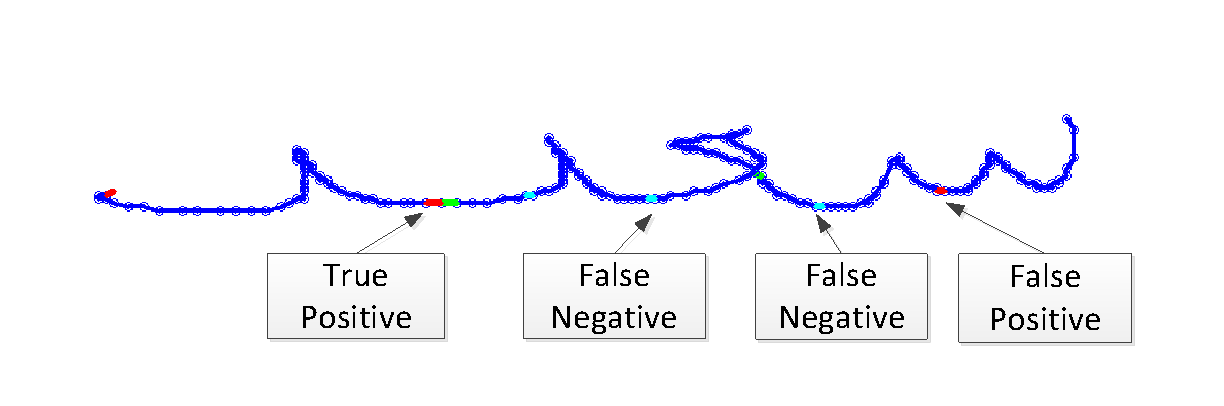
\includegraphics[width=0.6\textwidth]{./figures/sp_types}
\caption{SPs types.}
\label{fig:sp_types}
\end{figure}

\subsection{Analysis}
In this section we discuss common cases of incorrect segmentation.\\
\subsubsection{Over-segmentation}
\begin{itemize}
\item Several Arabic letters contain a horizontal region in their initial form which does not accommodate a SP, see Figure \ref{fig:candidate_in_no_horizontal}. 
We overcame this problem by adding the following rule: a POI is nominated only if the sub-stroke that spans from the beginning of the stroke to the POI has a high complexity measure.
\item Over-segmentation can also be caused by typing a letter in unusual form where it is spanned over several strokes. 
It happens mostly in the letter \RL{-m-}, \RL{-m} and in rare cases in the letter \RL{-.h-}. This issue will be addressed in a future work.
\end{itemize}

\subsubsection{Under-segmentation}
\begin{itemize}
\item Letter pairs that are not separated by HFs cause the system to miss POIs. This was partially solved by extending the notion of a letter to include such pairs. For example the pair \RL{lm} and \RL{l.h} .
\item In some cases, HFs were identified correctly but the corresponding POI were not selected in the third stage.
\end{itemize}

We have noticed that the absolute majority of the false negative (missed) SPs were actually identified as POIs in the first stage, but were not selected by the SSA.
In addition, differentiating between the main body of the letter \RL{-s-} and the main body of two consecutive \RL{-b-} letters is possible only when considering the additional strokes, thus both cases were considered to be correct.

\subsection{Segmentation Selection Algorithms Performance}
\label{subsec:ssa_performance}
It is apparent from the data in Table \ref{table:ss_algorithms_results}, that the SSA has a crucial effect on the system's performance. 
We tested several combinations of two SSAs in which the FSP is found by executing both SSAs independently and selecting the segmentation path with the smallest scoring. 

In Table \ref{table:ss_algorithms_results}, a combination of two algorithms is denoted by $\oplus$.

\begin{table}
\caption{SSAs Performance}
\begin{tabular}{ | c | c | c | c | c |}
\hline
\textbf{SSA} & \textbf{WP SR} & \textbf{WP RR} & S\textbf{P Precision} & \textbf{SP Recall}\\
\hline                 
  FSS & 76\% & 70\% & 85\% & 78\% \\ 
  \hline
  BSS & 79\% &  73\% & 84\%& 81\% \\
  \hline
  BFSS & 78\% & 72\% & 84\% & 80\%\\ 
  \hline
  GSS & 80\% & 74\% & 81\% & \bf{94}\% \\  
  \hline
  FSS$\oplus$BSS & \bf{82}\% & \bf{76}\% & \bf{89}\% & 82\%\\  
  \hline
  GSS$\oplus$BFSS & 81\% & 75\% & 83\% & 90\% \\
  \hline
\end{tabular}
\centering
\label{table:ss_algorithms_results} 
\end{table}

\subsection{Sample set size and distribution}
The letters is our training set are extracted from a database with a limited words diversity, thus, the distribution of the samples between the different classes is imbalanced. 
On one hand, it can be regarded as an advantage; since, the training set distribution reflects the a-priory probability of a letter appearance in the test set. 
On the other hand, a highly imbalanced training set is known to negatively affect many classification algorithms.
In the following experiment, we measure the effect of a large and imbalanced training set on the WP segmentation and recognition rates. 
It is done by gradually increasing the maximal allowed number of samples per class (letter and position).
 
The graph in Figure \ref{fig:num_letter_impact} shows convergence of the system's performance when the maximal number of samples is larger than 200 per class. 
Nevertheless, a miniature degradation is apparent, which is caused, probably, due to the increasing imbalance in the distribution of the training set.
In addition, it is evident that the recognition rate (RR) is more sensitive to small training set than the segmentation rate (SR).

\begin{figure}
\centering
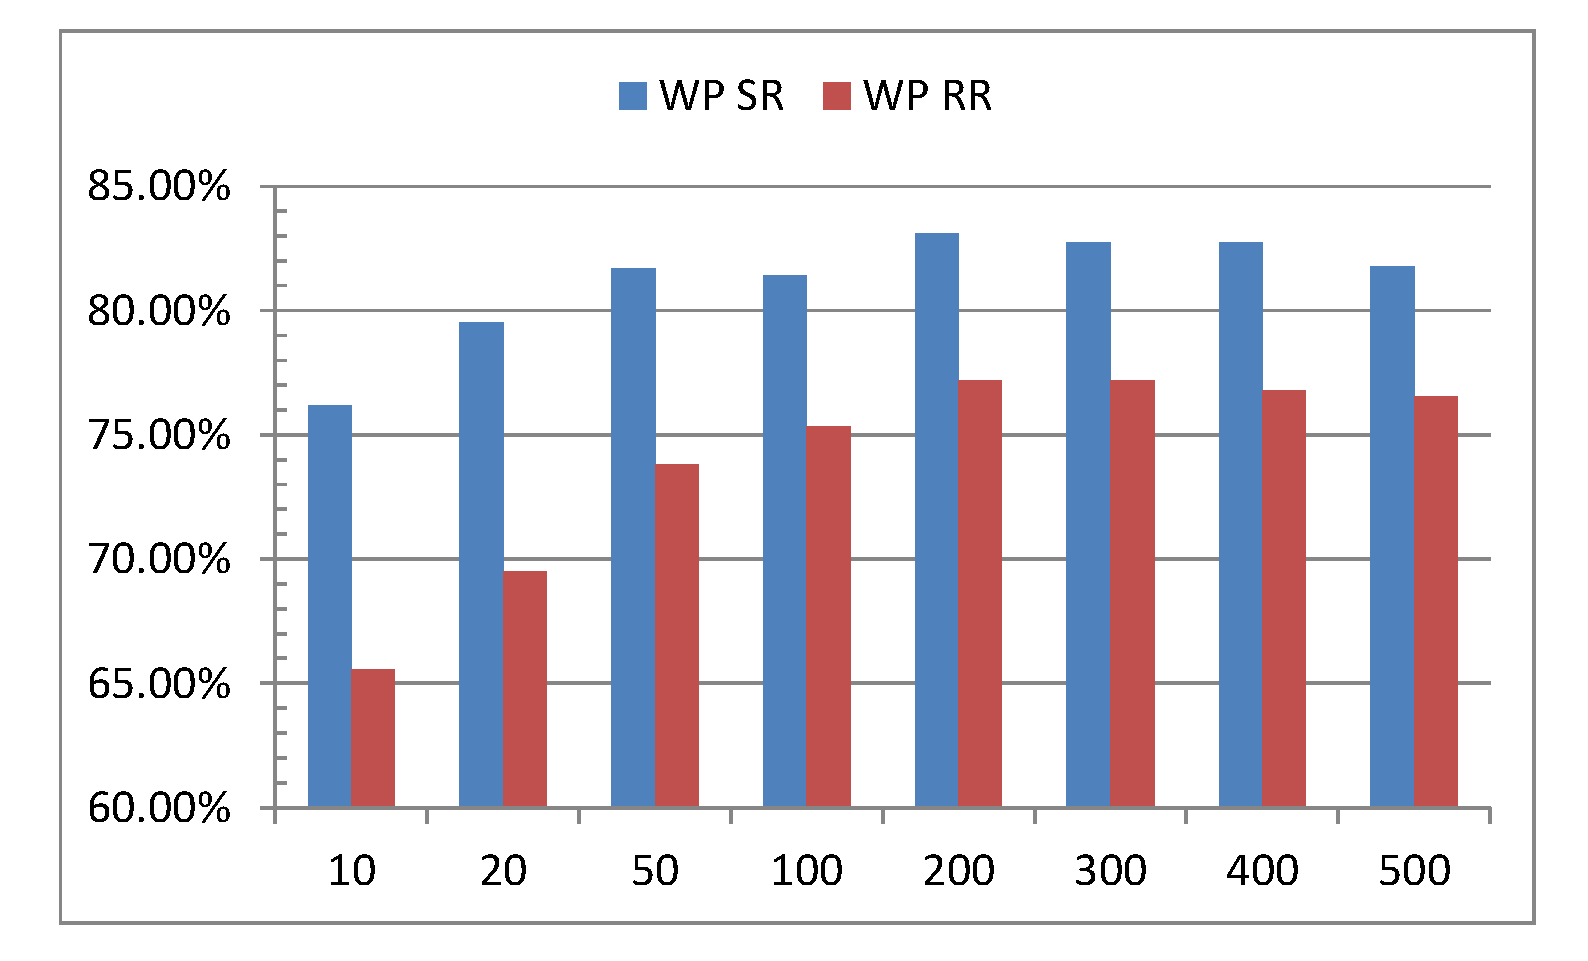
\includegraphics[width=0.7\textwidth]{./figures/num_letter_impact}
\caption{The impact of increasing the maximal number of samples per class on the segmentation and recognition rates.}
\label{fig:num_letter_impact}
\end{figure}

\section{WPs Recognition Using Characters Classification Information}
\label{sec:wps_recognition}
The segmentation and classification information obtained by a real-time segmentation system, can be used to significantly reduce the potential dictionary size and accelerate a later holistic recognition process.
In a dictionary-free environment, the classification information can be employed to dynamically build a class of different shapes for all possible WPs, as described below.
Following the real-time segmentation process, the $10$ top scored candidates of each character are recorded. 
These shapes are used to generate a complete list of all possible shape concatenation of the retrieved candidates. 
The obtained candidates represent different shapes of the same letter producing multiple shapes of the same WP. 
The cardinality of the generated list is $10^p$ where p is the predicted number of characters in the WP using the segmentation process. 
The large size of the generated list, which may exceed $100,000$ shapes, requires a similar process of embedding and dimensionality reduction, as described above, to generate a short list of candidates. 
The short list of candidates in the next step is matched against the queried WP using the original expensive and more accurate matching process. 
Using the proposed approach, the $10$ top WPs results yield a $98.1\%$ recognition rate. 
The recognition rate of the first top candidate dropped down to $90.8\%$. 
Using a voting process within the top five results gave a $94.7\%$ recognition rate. 

Analysing the failures of the misclassified samples shows that most recognition errors occur as a result of misclassifying a single character. 
In most cases the misclassified character is confused with a character having a very similar shape, which can be corrected using information retrieved by the associated additional stroke, such as the case of the letter \RL{-l} and the letter \RL{-n} in their handwritten form.

%\end{document}

%TODO:\\
%--------\\
%\begin{itemize}
%\item Comparing results with other researches.
%\item evaluate the speed affect of the kd-dtree.
%\end{itemize}
